\newpage
\chapter{Results}
\section{Empirical comparison of described models}\label{sec:results}
The models were tested on a set of job lists. Malapert's paper uses benchmark
job lists by \citet{daste1, daste2}. Since neither publication is
available online, I created my own set of randomized job lists for the purposes
of this paper, with $s_j, p_j \in [1, 20]$ and $d_j \in [1, 10n_j]$ where $n_j$ is
the number of jobs.\footnote{These instances will be updated to reflect the
feature distributions used in Daste et al.} Ten different sample job sets are
used per unique value of $n_j$. The times shown in figure \ref{fig:comp_times}
are averaged over those ten instances for each $n_j$.

The models were run on an i7 Q740 CPU in single-thread mode, with 8 GB RAM.
Solving was aborted after a time of 3600 seconds (1 hour).

The CP branch-and-bound model times out on most instances and is not shown here.
The CP model times out on one 12-job instance and gets progressively worse with
more jobs; similar to Malapert's original MIP model.
\begin{figure}
\centering

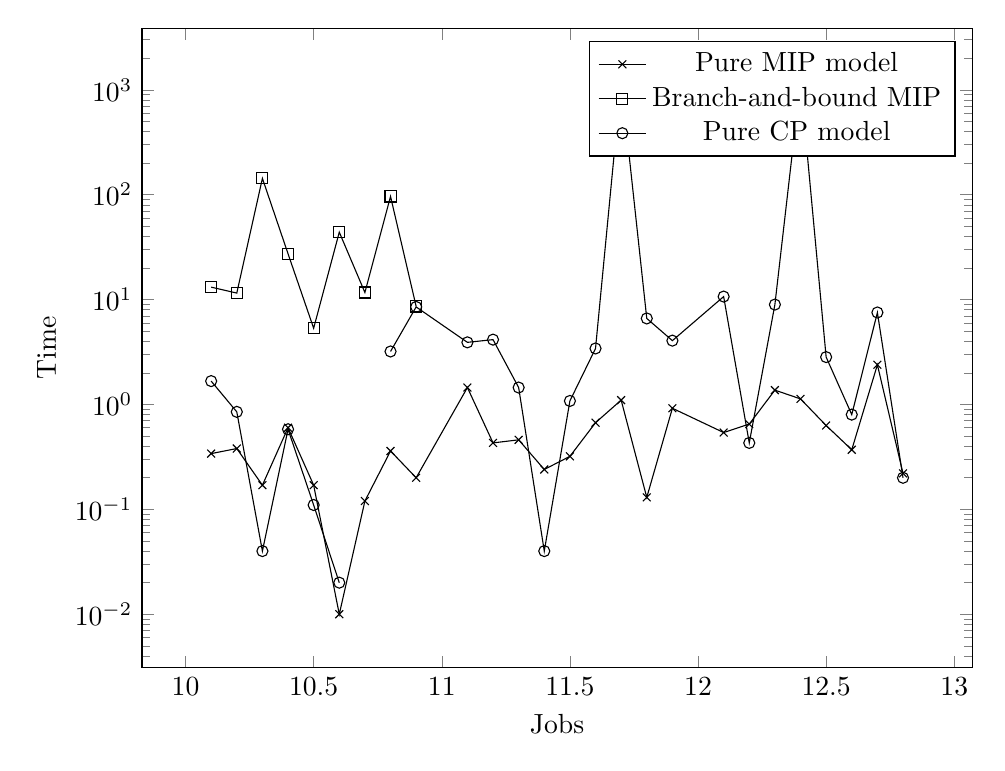
\begin{tikzpicture}
  \begin{semilogyaxis}[xlabel=Jobs, ylabel=Time, width=\textwidth,
  height=0.8\textwidth]
  \addplot[color=black, mark=x ] coordinates { % MIP model times
(10.1, 0.34)
(10.2, 0.38)
(10.3, 0.17)
(10.4, 0.6)
(10.5, 0.17)
(10.6, 0.01)
(10.7, 0.12)
(10.8, 0.36)
(10.9, 0.2)
(11.1, 1.45)
(11.2, 0.43)
(11.3, 0.46)
(11.4, 0.24)
(11.5, 0.32)
(11.6, 0.67)
(11.7, 1.1)
(11.8, 0.13)
(11.9, 0.92)
(12.1, 0.54)
(12.2, 0.65)
(12.3, 1.37)
(12.4, 1.13)
(12.5, 0.63)
(12.6, 0.37)
(12.7, 2.39)
(12.8, 0.22)
  };
  \addlegendentry{Pure MIP model}
  \addplot[color=black, mark=square] coordinates {
(10.1, 13.14)
(10.2, 11.53)
(10.3, 143.11)
(10.4, 27.34)
(10.5, 5.33)
(10.6, 43.9)
(10.7, 11.68)
(10.8, 96.27)
(10.9, 8.6)
  };
  \addlegendentry{Branch-and-bound MIP}
  \addplot[color=black, mark=o] coordinates {
(10.1, 1.67)
(10.2, 0.85)
(10.3, 0.04)
(10.4, 0.58)
(10.5, 0.11)
(10.6, 0.02)

(10.8, 3.2)
(10.9, 8.51)
(11.1, 3.91)
(11.2, 4.15)
(11.3, 1.45)
(11.4, 0.04)
(11.5, 1.08)
(11.6, 3.42)
(11.7, 1200)
(11.8, 6.61)
(11.9, 4.06)
(12.1, 10.68)
(12.2, 0.43)
(12.3, 8.96)
(12.4, 1200)
(12.5, 2.83)
(12.6, 0.8)
(12.7, 7.53)
(12.8, 0.2)
};
  \addlegendentry{Pure CP model}
  \end{semilogyaxis}
\end{tikzpicture}

\caption{Comparison of CPU time used by different models.}
\label{fig:comp_times}
\end{figure}




